\documentclass[anonymous,sigconf,9pt]{acmart}

\usepackage{microtype}
\usepackage{tikz,pgfplots}
\usetikzlibrary{arrows.meta}
\usepgfplotslibrary{groupplots}
\usepgfplotslibrary{external}
\usepgfplotslibrary{colorbrewer}
\pgfplotsset{cycle list/Set1}
\usepgfplotslibrary{fillbetween}a
\pgfplotsset{compat=1.18}
\pgfplotsset{
    tick align=outside,
    tick pos=left,
    xmajorgrids,
    x grid style={white},
    ymajorgrids,
    y grid style={white},
    axis line style={white},
    axis background/.style={fill=white!89.803921568627459!black},
    legend style={draw=none, fill=none},
    legend cell align=left,
}
\pgfkeys{/pgf/number format/.cd, 1000 sep={\,}}

\pgfplotsset{
    log x ticks with fixed point/.style={
        xticklabel={
            \pgfkeys{/pgf/fpu=true}
            \pgfmathparse{2^\tick}%
            \pgfmathprintnumber[fixed relative, precision=4]{\pgfmathresult}
            \pgfkeys{/pgf/fpu=false}
        }
    },
    log10 x ticks with fixed point/.style={
        xticklabel={
            \pgfkeys{/pgf/fpu=true}
            \pgfmathparse{10^\tick}%
            \pgfmathprintnumber[fixed relative, precision=3]{\pgfmathresult}
            \pgfkeys{/pgf/fpu=false}
        }
    },
    log y ticks with fixed point/.style={
        yticklabel={
            \pgfkeys{/pgf/fpu=true}
            \pgfmathparse{2^\tick}%
            \pgfmathprintnumber[fixed relative, precision=4]{\pgfmathresult}
            \pgfkeys{/pgf/fpu=false}
        }
    }
}

\begin{document}

\begin{figure*}[tbp]
\centering
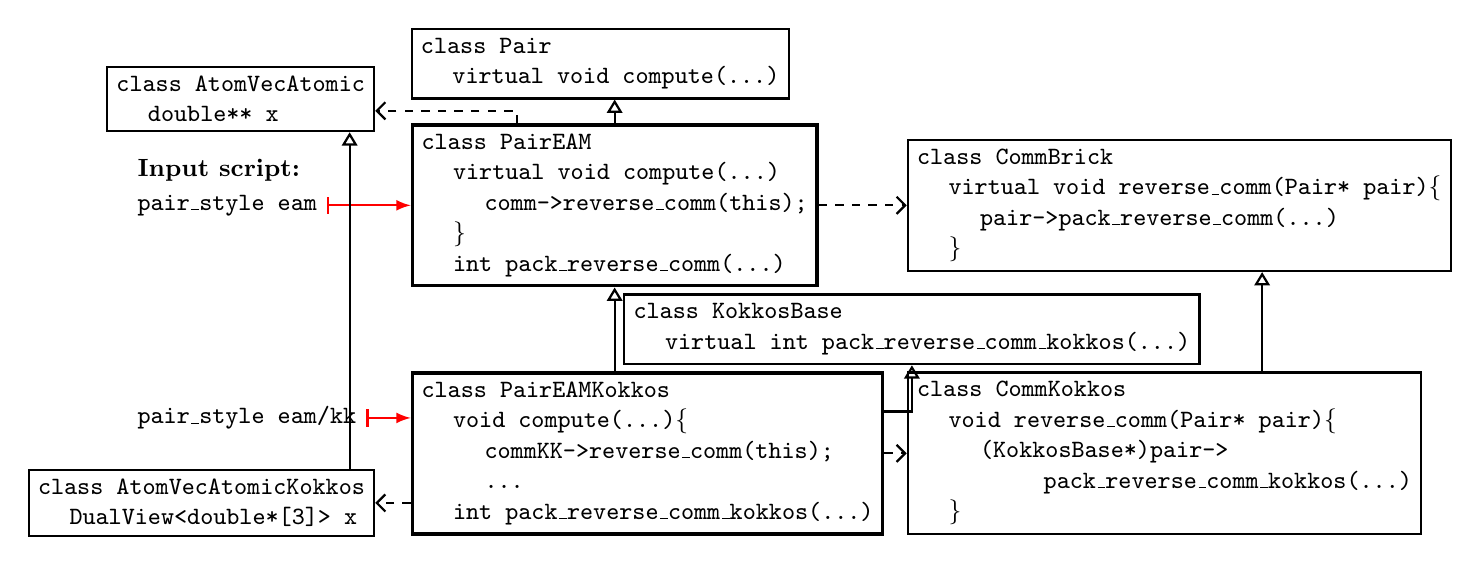
\begin{tikzpicture}[x=0.9cm,y=0.9cm,thick,>=latex,font=\small]
    \draw (0,0) node[anchor=west] (paiream) {\texttt{pair\_style eam}};
    \draw (0,-3) node[anchor=west] (paireamkk) {\texttt{pair\_style eam/kk}};
    \draw (0,0.5) node[anchor=west] (input) {\textbf{Input script:}};

    \draw (4,0) node[very thick,draw,anchor=west,align=left] (pair) {\texttt{class PairEAM}\\ \hspace{0.4cm}\texttt{virtual void compute(...)}\\
        %\hspace{0.8cm}\texttt{...}\\
        \hspace{0.8cm}\texttt{comm->reverse\_comm(this);}\\
        %\hspace{0.8cm}\texttt{...}\\
        \hspace{0.4cm}\texttt{\}}\\
    \hspace{0.4cm}\texttt{int pack\_reverse\_comm(...)}};
    \draw (4,-3.5) node[very thick, draw,anchor=west,align=left] (pairkk) {\texttt{class PairEAMKokkos}\\
        \hspace{0.4cm}\texttt{void compute(...)\{}\\
        %\hspace{0.8cm}\texttt{...}\\
        \hspace{0.8cm}\texttt{commKK->reverse\_comm(this);}\\
        \hspace{0.8cm}\texttt{...}\\
        %\hspace{0.4cm}\texttt{\}}\\
        \hspace{0.4cm}\texttt{int pack\_reverse\_comm\_kokkos(...)}};

    \draw[<-|, red] (pair.west |- paiream.east) -- (paiream.east); 
    \draw[<-|, red] (pairkk.west |- paireamkk.east) -- (paireamkk.east); 

    \draw (4,2.0) node[draw,anchor=west,align=left] (pairbase) {\texttt{class Pair}\\ \hspace{0.4cm}\texttt{virtual void compute(...)}};
    \draw (7,-1.75) node[draw,anchor=west,align=left] (kkbase) {\texttt{class KokkosBase}\\ \hspace{0.4cm}\texttt{virtual int pack\_reverse\_comm\_kokkos(...)}};

    \draw[{Triangle[open]}-] (pairbase.south -| pair.north) -- (pair.north);
    \draw[-{Triangle[open]}] (pairkk.north -| pair.south) -- (pair.south);
    \draw[{Triangle[open]}-]  (kkbase.south) |- (pairkk.10);

    \draw (3.5,1.5) node[draw, align=left, anchor=east] (atom) {\texttt{class AtomVecAtomic}\\ \hspace{0.4cm}\texttt{double** x}};  
    \draw (3.5,-4.2) node[draw, align=left, anchor=east] (atomkk) {\texttt{class AtomVecAtomicKokkos}\\ \hspace{0.4cm}\texttt{DualView<double*[3]> x}};  
    
    \draw[{Triangle[open]}-] (atom.345 -| atomkk.13) -- (atomkk.13);
    \draw[dashed,-{Straight Barb[]}] (pair.140) |- (atom.355);
    \draw[dashed,-{Straight Barb[]}] (pairkk.west |- atomkk.east) -- (atomkk.east);
    
    \draw (11,0) node[draw, align=left, anchor=west] (comm) {\texttt{class CommBrick}\\
        \hspace{0.4cm}\texttt{virtual void reverse\_comm(Pair* pair)\{}\\
        %\hspace{0.8cm}\texttt{...} \\
        \hspace{0.8cm}\texttt{pair->pack\_reverse\_comm(...)} \\
        %\hspace{0.8cm}\texttt{...}  \\
        \hspace{0.4cm}\texttt{\}}
    };
    \draw (11,-3.5) node[draw, align=left, anchor=west] (commkk) {\texttt{class CommKokkos}\\
        \hspace{0.4cm}\texttt{void reverse\_comm(Pair* pair)\{}\\
        %\hspace{0.8cm}\texttt{...} \\
        \hspace{0.8cm}\texttt{(KokkosBase*)pair->} \\ 
        \hspace{1.5cm} \texttt{pack\_reverse\_comm\_kokkos(...)} \\
        %\hspace{0.8cm}\texttt{...}  \\
        \hspace{0.4cm}\texttt{\}}
    };  
    \draw[dashed,-{Straight Barb[]}] (pair.east |- comm.west) -- (comm.west);
    \draw[dashed,-{Straight Barb[]}] (pairkk.east |- commkk.west) -- (commkk.west);
    \draw[{Triangle[open]}-] (comm.320 -| commkk.40) -- (commkk.40);
\end{tikzpicture}
\caption{Mapping (red arrows) from user input script commands to LAMMPS class hierarchy and how the classes interact within and outside of the KOKKOS package. The pair styles operate on atomic data stored as pointers in \texttt{AtomVecAtomic} and \texttt{Kokkos::DualView}s in \texttt{AtomVecAtomicKokkos}, with the pointer in the former aliased to the CPU mirror of the latter. The EAM pair style requires additional communication, which is performed with calls to the LAMMPS communication classes.}\label{fig:flow}
\end{figure*}
\end{document}

